%!TEX root = ./../main.tex
\section{Prototyp}\label{section:prototyp}
Zur Lösung der Aufgabenstellung haben wir einen lauffähigen Prototypen entwickelt, der die Machbarkeit der Analyse demonstriert.
Dafür haben wir die im vorhergehenden Kapitel genannten Technologien eingesetzt. Die Details zu den jeweils entstandenen
Anwendungen stellen wir in diesem Kapitel vor.

\begin{figure}[h]
    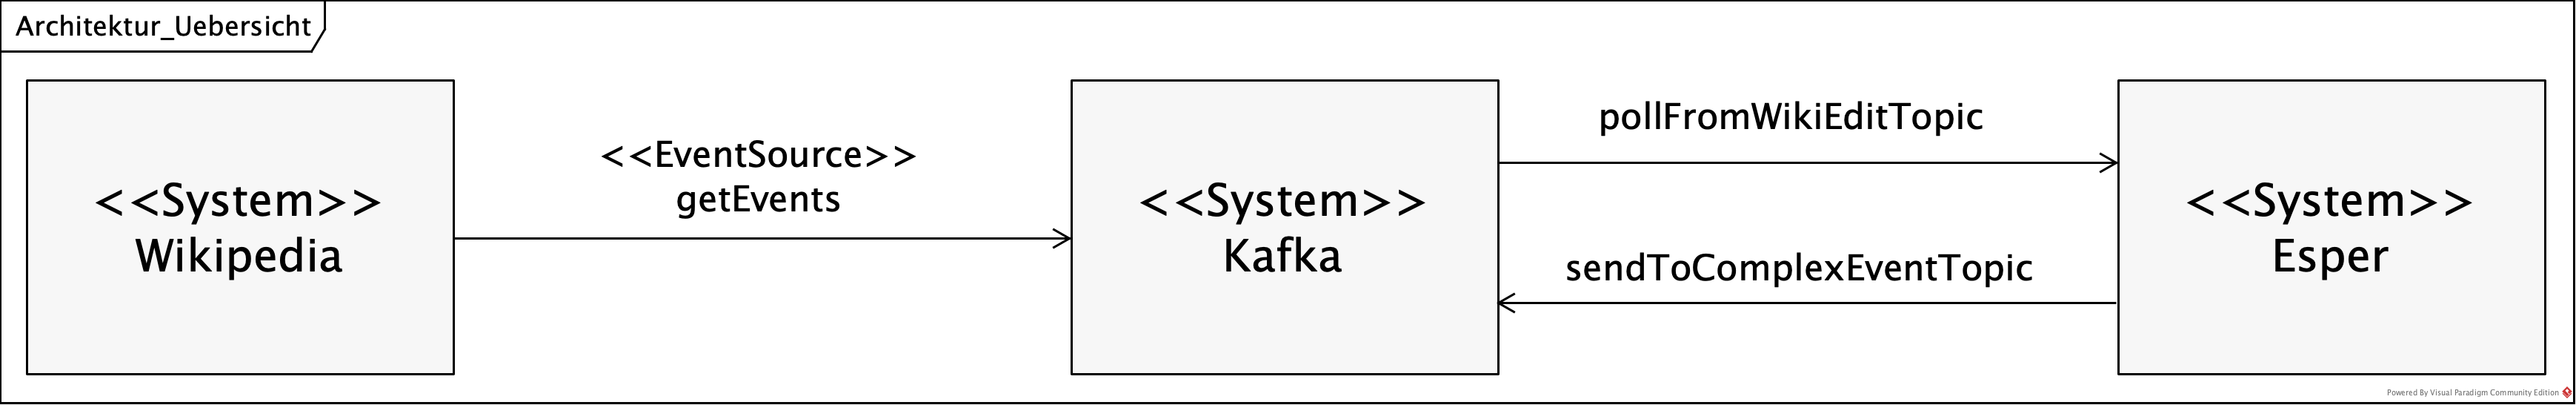
\includegraphics[width=.5\textwidth]{images/Architektur_Uebersicht.png}
    \caption{Architekturübersicht}
    \label{fig:architektur_uebersicht}
\end{figure}

Abbildung \ref{fig:architektur_uebersicht} zeigt die Teilsysteme und deren Interaktion untereinander.

% Abbildung \ref{fig:architektur_uebersicht} zeigt bisher nur eine sehr rudimentäre Übersicht und soll als Grundlage dienen.
% Die Verbindung zwischen Esper und Kafka muss noch genauer werden: Protokoll, senden von komplexen Events in neue Kafka-Topics.

\subsection{Collection-Tier: Wikipedia}
Wie zuvor beschrieben, stützt sich unser System auf Daten von Wikipedia. Wir nutzen den Recent-Changes-Stream, der
Events zu neu erstellten, aktualisierten und gelöschten Wikipedia-Seiten enthält \cite{WikimediaManual}.
Der Quellcode \ref{WikipediaRecentChangeJSON} zeigt einen Ausschnitt eines solchen Events.
Es sind nur die Attribut abgebildet, die in einem der nachfolgenden Teilsysteme relevant sind.

\begin{lstlisting}[label=WikipediaRecentChangeJSON,caption=Wikipedia Recent-Change-Event,language=json,firstnumber=1,captionpos=b]
{
    "bot": false,
    "comment": "/* Politischer Werdegang */",
    "id": 269108829,
    "meta": {
        "uri": "https://de.wikipedia.org/wiki/Ingeborg_H%C3%A4ckel",
        "partition": 0,
        "offset": 1329388977
    },
    "timestamp": 1547910734,
    "title": "Ingeborg H\"ackel",
    "user": "Eszet2000",
    "wiki": "dewiki"
}
\end{lstlisting}

Die beiden Parameter \code{offset} und \code{uri}, innerhalb des \code{meta}-Objektes, stammen aus einem Kafka-System
und dienen der Wiederaufnahme eines abgebrochenen Streams \cite{WikimediaManual}. Wikipedia setzt intern Apache Kafka als Messaging-System ein.
Nach außen nutzt Wikipedia EventStreams. Das ist ein Webservice der kontinuierliche Datenströme mit strukturierten Daten
über HTTP sendet\footnote{https://wikitech.wikimedia.org/wiki/EventStreams}. Die Basis-Technologie dessen, ist
das Server-Sent Event (SSE) Protokoll. Der Recent-Changes-Stream ist ein solcher Stream und kann über eine Client-Bibliothek
konsumiert werden.

Wie im vorherigen Kapitel beschrieben, werden Daten vom Collection-Tier mithilfe eines der aufgelisteten Pattern übertragen.
SSE funktioniert nach dem One-Way-Pattern, indem eine HTTP-Verbindung erzeugt wird um Nachrichten zu empfangen \cite{EventSource_SSE}.

\subsection{Implementierungsdetails zum Messaging-Queuing-Tier: Kafka}
Im Messaging-Queuing-Tier setzen wir Apache Kafka in der Version 2.1 ein, um die im Collection-Tier beschriebenen Wikipedia-Events
in unser eigenes Messaging-System zu überführen. Hierfür haben wir eine Java-Anwendung entwickelt, in der die folgenden
Schritte nacheinander ausgeführt werden:
\begin{enumerate}
    \item \textit{Kafka Initialisierung.} Den Host des Bootstrap-Servers setzen um eine Verbindung zu erzeugen.
    Als Key- und Value-Serialisierer setzen wir
    jeweils den \code{StringSerializer} von Kafka ein. Das heißt, die Events werden als JSON-String in das Topic \code{wikiEdit}
    eingespeist. Zum Senden von Events erzeugen wir ein Producer-Objekt mit dem passenden Typ \code{Producer<String, String>}.
    An dieser Stelle war die Überlegung, anstelle eines String-Serialisierers für den Wert des Producers,
    einen eigenen Serialisierer für die \code{WikipediaEditEvent}-Klasse einzusetzen -- Details hierzu in Abbildung \ref{fig:class_diagram_eventtypes}. Wir entschieden uns aber für den
    String-Serialisierer, da Wikipedia die Events auch als JSON-String überträgt und wir in Kafka selbst
    keine weiteren Operationen an den Daten vornehmen. Eine mögliche Operation könnte ein Filter sein.
    Aber das einzige Ziel von Kafka soll die Persistierung und Weitergabe von Daten sein. Dafür ist keine De-/Serialisierung in
    einem bestimmten Typen notwendig. Ein weiterer Grund ist die Verschiebung der Komplexität aus der Kafka-Anwendung
    in die Consumer-Anwendungen. Dadurch bleibt die Kafka-Anwendung so leichtgewichtig wie möglich.
    \item \textit{Erzeugung eines EventHandlers.} Für das Empfangen von EventSource-Nachrichten nutzen wir die Java-Bibliothek
    \textit{okhttp-eventsource}\footnote{https://github.com/launchdarkly/okhttp-eventsource}. Zur Verarbeitung der Events
    \code{onOpen}, \code{onClose}, \code{onMessage}, \code{onComment} und \code{onError} muss das Interface \code{EventHandler} von
    \textit{okhttp-eventsource} implementiert werden.
    \item \textit{Erzeugung und Starten einer EventSource.} Mit der Stream-URI der Wikipedia-EventSource (für die Recent-Changes ist das: https://stream.wikimedia.org/v2/stream/recentchange)
    und des implementierten EventHandler-Interfaces
    kann ein \code{EventSource}-Objekt erzeugt werden. Das Objekt dient dem Starten und Beenden eines EventSource-Streams.
    Die Daten werden dann, wie zuvor beschrieben, durch das SSE-Protokoll von Wikipedia an die Anwendung gesendet.
    \item \textit{Beim Eintreffen eines Events: Senden einer Nachricht in ein Kafka-Topic.} Tritt ein Wikipedia-Event auf,
    wird die \code{onMessage}-Methode des implementierten EventHandlers-Interface aufgerufen. Der zweite Parameter enthält die Daten
    des aufgetretenen Events. Der Zugriff auf die als JSON-String codierte Nachricht erfolgt über die \code{getDate()}-Methode.
    Diese Daten sendet die Anwendung, über den zuvor erzeugten Producer, ohne eine weitere
    Verarbeitung in das Kafka-Topic \code{wikiEdit}.
\end{enumerate}

Die Konfiguration der Kafka-Topics ist sehr einfach gehalten, da es sich bei der Anwendung nur um einen Prototypen handelt.
Wir nutzen nur ein Topic mit dem Namen \code{wikiEdit}. Da die Anwendung auf nur einem Server läuft, setzen wir auch nur
eine Partition ein und haben keine Replikation. Durch die Eigenschaften von Kafka steht einer Skalierung der Kafka-Anwendung
auf mehrere parallel-arbeitende Server nichts im Weg.

\subsection{Implementierungsdetails zum Analysis-Tier: Esper}
In unserer Esper-Anwendung, die das Hauptsystem des Analysis-Tier ist, nutzen wir Esper in Version 7.1
als Complex-Event-Processing-Werkzeug.
Zur Verarbeitung der Wikipedia-Events haben wir zwei Lösungen umgesetzt, da die erste Lösung nicht
zum Erreichen der Ziele führte. Für ein besseres Verständnis geben wir einen kurzen Überblick über den gemeinsamen Aufbau beider
Lösungen. Danach beschreiben wir die Details und Unterschiede der jeweiligen Lösungen und analysieren diese hinsichtlich der
Zielerfüllung.
In unserer Esper-Anwendung sind wir im Allgemeinen wie folgt vorgegangen:

\begin{enumerate}
    \item \textit{Esper Initialisierung.} Die Initialisierung von Esper besteht aus der Erzeugung einer \code{Configuration},
    der Erstellung und dem Starten von EPL-Statements, sowie dem Erzeugen von Listener-Klassen.
    \item \textit{Kafka initialisieren und starten.} Um die Daten aus dem Messaging-Queuing-Tier zu bekommen haben wir einen
    \code{KafkaConsumer<String, String>} implementiert.
    Wir pollen in einer Endlosschleife alle 10 Millisekunden die Daten vom Kafka-Topic \code{wikiEdit}. Bei den empfangenen Daten
    handelt es sich um einen String, der JSON enthält. Mithilfe der Gson-Bibliothek\footnote{https://github.com/google/gson}
    konvertieren wir die JSON-Strings in Java-Objekte. Die daraus resultierenden Java-Objekte senden wir wiederum in das
    Esper-System, damit darauf die EPL-Statements angewandt werden können.
    \item \textit{Aktion ausführen, sobald das Muster erfüllt ist.} Ist das Muster erfüllt, wird die \code{update}-Methode der Listener-Klasse
    aufgerufen. Es werden die alten und neuen Events übergeben. Daraus kann eine Aktion erfolgen, z.\,B. dass erzeugen eines neuen
    komplexen Events.
\end{enumerate}


\subsubsection{Lösung 1}
In unserer ersten Lösung war es unser Ziel, relevante Events durch die Modellierung geeigneter Ereignistypen zu detektieren.
Ein relevantes Event besteht für uns aus einer definierten \textit{Anzahl an Benutzer} die in einem
definierten \textit{Zeitraum} eine definierte \textit{Menge an Bearbeitungen} an einer Wikipedia-Seite vornehmen.
Zur weiteren Konkretisierung zeigt Quellcode \ref{Solution1_EPL1} das erste EPL-Statement. Hierbei werden
5 aufeinanderfolgende \code{WikipediaEditEvent}, die kein Bot sind, von unterschiedlichen Benutzern stammen
und die gleiche URI aus der deutschsprachigen Wikipedia haben. Desweiteren wird mit der \code{checkWithin}-Methode
geprüft, ob die Events \code{w2} bis \code{w5} jeweils den definierten Zeitabstand von 600 Sekunden nicht überschreiten.
In Esper werden diese Methoden Single-Row-Functions genannt. Diese müssen in der \code{Configuration} angegeben werden
und es handelt sich dabei um eine einfache Java-Methode, die einen \code{Boolean} als Rückgabetyp hat.

\begin{lstlisting}[label=Solution1_EPL1,caption=Lösung 1: EPL-Statement 1,language=epl,firstnumber=1,captionpos=b]
insert into WikipediaEditEventFive
select w1, w2, w3, w4, w5
from pattern[
    every
    w1=WikipediaEditEvent(bot = false, wiki='dewiki') ->
    ...
    w5=WikipediaEditEvent(w5.meta.uri = w1.meta.uri, bot = false, user <> w1.user, user <> w2.user, user <> w3.user, user <> w4.user, checkWithin(w1, w5, 600))
]
\end{lstlisting}

Der Zugriff auf die Attribute der \code{WikipediaEditEvent}-Klasse erfolgt über Getter und Setter, die im Klassendiagramm
der Abbildung \ref{fig:class_diagram_eventtypes} zur besseren Lesbarkeit nicht angegeben wurden.
Ist das Muster aus dem Quellcode \ref{Solution1_EPL1} erfüllt, wird ein neues Event des Typs \code{WikipediaEditEventFive}
eingefügt. Bei der Erzeugung werden dem Konstruktor die selektierten Objekte \code{w1} bis \code{w5} übergeben.

\begin{figure}[h]
    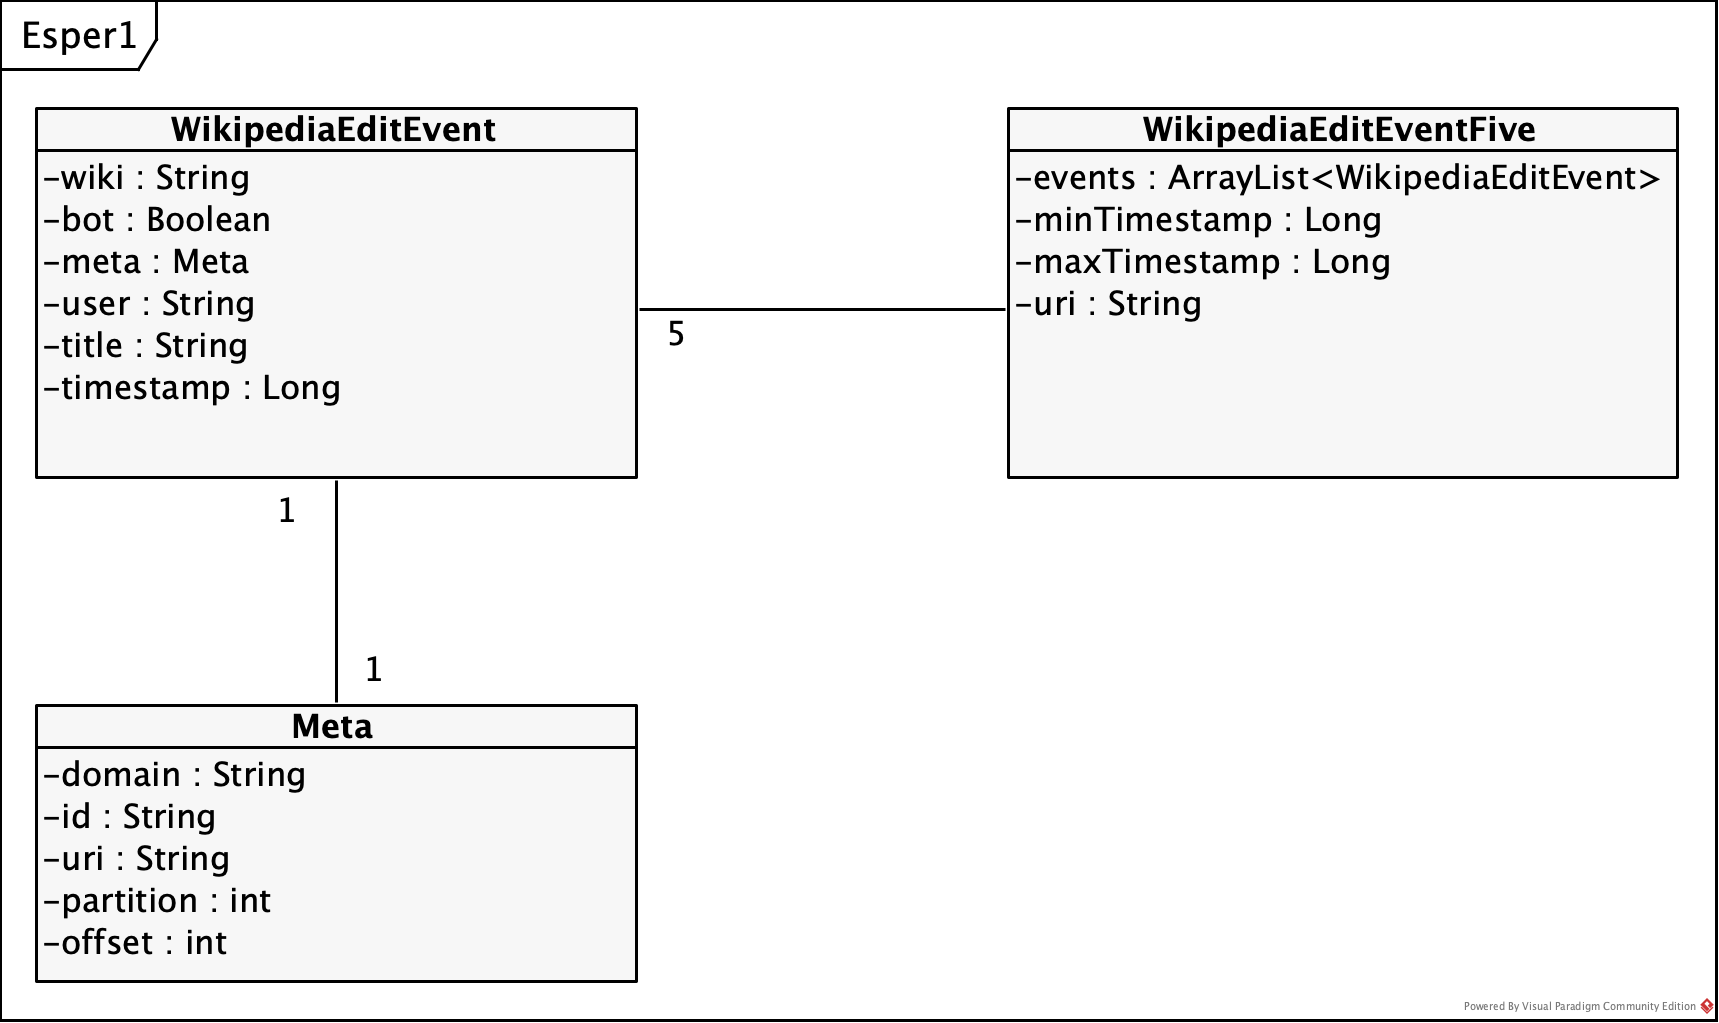
\includegraphics[width=.5\textwidth]{images/Esper1.png}
    \caption{Klassendiagramm der zwei Ereignistypen WikipediaEditEvent, WikipediaEditEventFive und der Helferklasse Meta}
    \label{fig:class_diagram_eventtypes}
\end{figure}

Das zweite EPL-Statement ist von der Funktionsweise her analog zum ersten. Das Muster besteht jedoch nicht aus
5 aufeinanderfolgenden \code{WikipediaEditEvent}, sondern aus
4 aufeinanderfolgenden \code{WikipediaEditEventFive} die in einem Zeitraum von 20 Minuten aufgetreten sind.

Die beiden Zahlen, 4 und 5 sind durch Ausprobieren ermittelt worden. Das zeigt sehr deutlich, dass das weder eine
effiziente noch eine sehr erfolgreiche Lösung für unsere Aufgabe ist.
Das Problem liegt an den sehr unterschiedlichen Menge an Bearbeitungen.
Denn es gibt Wikipedia-Seiten, die dauerhaft einer großen Menge an Aktualisierungen unterworfen sind und wiederum andere Wikipedia-Seiten, die
nur sehr sporadisch aktualisiert werden. Aus diesen Gründen ist es uns mit dieser Herangehensweise
nicht gelungen eine Vereinheitlichung, für relevante Events, über alle Wikipedia-Seiten hinweg zu finden.

\subsubsection{Lösung 2}
Die Probleme der Lösung 1 führten dazu, dass wir einen Ansatz verfolgten, bei dem die Betrachtung einzelner Seiten mehr im Fokus steht.
In Lösung 2 sind wir ein Stück weg vom Website Activity Tracking, hin zur Anomalieerkennung gegangen. Das zeigt sich auch in der
Architektur aus Abbildung \ref{fig:architektur_uebersicht}, in der neben der Esper-Anwendung auch ein Aufruf eines
Burst-Detection-Algorithmus abgebildet ist.

Konkret sieht die Implementierung so aus, dass wir 100 Events einer URI aggregieren und darauf wenden wir den Burst-Detection-Algorithmus an.
Das ermöglicht es uns Anomalien -- ein starker Anstieg der Anzahl der Aktualisierungen -- einzelner URIs zu betrachten.
Der Quellcode \ref{Solution2_EPL1} zeigt das EPL-Statement hierzu. Es wird eine URI-Partitionierung mithilfe eines
Kontexts erstellt. Damit wird das Muster zur Aggregation der 100 Events je URI, mit einem Batch-Window, umgesetzt.

\begin{lstlisting}[label=Solution2_EPL1,caption=Lösung 2: EPL-Statement 2,language=epl,firstnumber=1,captionpos=b]
create context GroupByUri partition by meta.uri from WikipediaEditEvent

context GroupByUri
select *
from WikipediaEditEvent(bot=false , wiki='dewiki').win:length_batch(100)
\end{lstlisting}

Wird das Muster erkannt, werden die Timestamps der 100 selektierten Events an die REST-Schnittstelle des BurstDetection-Service gesendet.
Dieser wendet einen Burst-Detection-Algorithmus auf die Daten an und gibt ein Array mit \textquotedblleft Ebenen\textquotedblright zurück.
Die Ebene 0 entspricht hierbei dem gesamten Datensatz von 100 Events. Je höher die Ebene, desto stärker und klarer abgegrenzt ist die
Anomalie bzw. der Burst. Für uns hat sich gezeigt, dass Events aber der Ebene 2 einem relevanten Ereignis sehr nahe kommen.

Betrachtet man die 100 Events der Wikipedia-Seite der Handball-Weltmeisterschaft der Männer 2019\footnote{https://de.wikipedia.org/wiki/Handball-Weltmeisterschaft\newline{}\_der\_M\%C3\%A4nner\_2019}
in dem Zeitraum vom 25. Juni 2018 12:44 Uhr bis zum 12. Januar 2019 17:06 Uhr, ergibt sich folgende Ausgabe:

\begin{lstlisting}[label=Solution2_Layers,caption=Ebene 0\, 1 und 2 der Burst-Detectionen,language=epl,firstnumber=1,captionpos=b]
[[0, 1529923440000, 1547309160000], [1.0, 1546853700000, 1547309160000], [2.0, 1547136540000, 1547243280000]]
\end{lstlisting}

Die Ebene 0 entspricht hier allen 100 Events, die Ebene 1 geht vom 07. Januar 2019 10:35 Uhr bis zum 12. Januar 2019 17:06 Uhr und die
Ebene 2 geht vom 10. Januar 2019 17:09 Uhr bis zum 11. Januar 2019 22:48 Uhr. Je höher die Ebene, desto kleiner und auch
relevanter wird ein Bereich. Relevant heißt, dass in diesem Bereich mehr Events als sonst aufgetreten sind -- ein Burst.
Das Beispiel zeigt also, dass wir durch die Lösung 2 für einzelne Wikipedia-Seiten relevante Ereignisse ableiten können.

\subsection{BurstDetection-Implementierung}
Die Burst-Detection ist in Python geschrieben. Es handelt sich hierbei um ein REST-Interface mit einem Endpunkt,
der beim Aufruf lediglich als Wrapper für den Aufruf der Burst-Detection fungiert. Die Burst-Detection wird durch ein
zusätzliches Python-Package eingefügt und ist auch austauschbar.